\documentclass{article}

\usepackage{graphicx}
\usepackage{subfig}
\usepackage{amsmath}
%\usepackage{amsmath,rotating}

\title{Laminar, Two-dimensional Couette Flow}

\date{}

\begin{document}

\maketitle

\section{Introduction}
This case provides a description for two-dimensional Couette flow
with constant properties, and a zero pressure gradient.

\section{Domain}
The two-dimensional geometry for this tutorial is captured in 
Figure~\ref{fig:geom} where the rectangular domain is defined by the 
height, $H$, and length, $L$. The streamwise and vertical velocity are 
defined as $u_x$ and $u_y$, respectively.

The top surface is a no-slip wall boundary specification $u_x = u_b$, where $u_b$ is a bulk velocity
of the top moving wall and $u_y = 0$. The bottom surface is also a no-slip wall boundary 
specifications with $u_x = u_y = 0$.
Finally, the left and right surfaces are periodic. In absence of any 
external body forces, the flow is aligned to the x-axis and is 
strictly a function of the vertical-dimension, $y$, i.e., $u_x = f(y)$.

\begin{figure}[!htbp]
  \centering
  {
   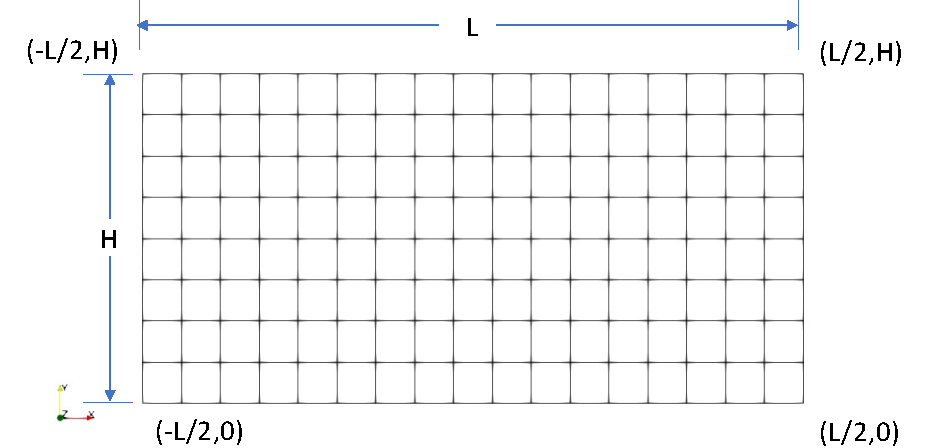
\includegraphics[height=2.0in]{images/2d_quad9_couette_geom.pdf}
  }
  \caption{Two-dimensional couette flow in which the height is 2 m and length, 1 m}
  \label{fig:geom}
\end{figure}

\section{Theory}
The variable-density low-Mach equation set is defined by the continuity and momentum equation,

\begin{align}
  \frac {\partial \rho }{\partial t} + \frac{ \partial \rho u_j}{\partial x_j} = 0.
\label{eq:contEq}
\end{align} 

\begin{align}
  \frac {\partial \rho u_i }{\partial t} + \frac{ \partial \rho u_j u_i}{\partial x_j} 
-\frac{\partial \sigma_{ij}}{\partial x_j} = 0.
\label{eq:momEq}
\end{align}
%
In the above equation, $\rho$ is the fluid density and $u_j$ is the fluid velocity. 
The stress tensor is provided by
\begin{align}
\sigma_{ij}  = 2 \mu S^*_{ij} - P \delta_{ij},
\end{align}
%
where the traceless rate-of-strain tensor is defined as
\begin{align}
S^*_{ij}  = S_{ij} - \frac{1}{3} \delta_{ij} S_{kk} \nonumber
		     = S_{ij} - \frac{1}{3} \frac{\partial  u_k }{\partial x_k}\delta_{ij}.
\end{align}
In a low-Mach flow, the above pressure, $P$, is the perturbation about the thermodynamic
pressure, $P^{th}$. 

\subsection{Analytical Velocity Profile}
Given the assumptions provided in the introduction, the streamwise velocity equation reduces to,

\begin{align}
   \mu \frac{d^2 u_x}{dy^2} = 0.
\label{eq:simpEq}
\end{align}
We note that a more interesting Couette flow can be derived in the presence of a constant pressure 
gradient. Activation of a non-zero dynamic viscosity, Equation~\ref{eq:simpEq} can be 
integrated twice to obtain,

\begin{align}
  u_x(y) = k_1 y + k_2,
\label{eq:simpEqWithK}
\end{align}
where $k_1$ and $k_2$ are constants of integration that are obtained through the 
application of boundary conditions, $u_x(y=0) = 0$ and  $u_x(y=H) = u_b$. Therefore,
the final expression for the streamwise velocity is simply a linear function of vertical
distance,

\begin{align}
  u_x(y) = \frac{u_b}{H}y.
\label{eq:simpleEqWithoutK}
\end{align}

\section{Results}


Let us test a simulation in which a the Reynolds number based on height of the domain,
assuming the properties of water ($\rho = $1000 $kg/m^3$ and $\mu = $8.9e-4 $Pa-s$)
at a bulk top velocity of $u_b = $1e-3 $m/s$, is approximately 1236.

\begin{align}
  Re = \frac{\rho u^b H}{\mu}.
\label{eq:muForm}
\end{align}

\subsection{Simulation Specification and Results}

The mesh exercised activates a Quad9 topology, thereby exercising a
quadratic underlying basis that yields a nominal third-order spatial accurate
simulation.

In Figure~\ref{fig:results}, results are provided for the specifications
provided above.

\begin{figure}[!htbp]
  \centering
  \subfloat[]
  {
   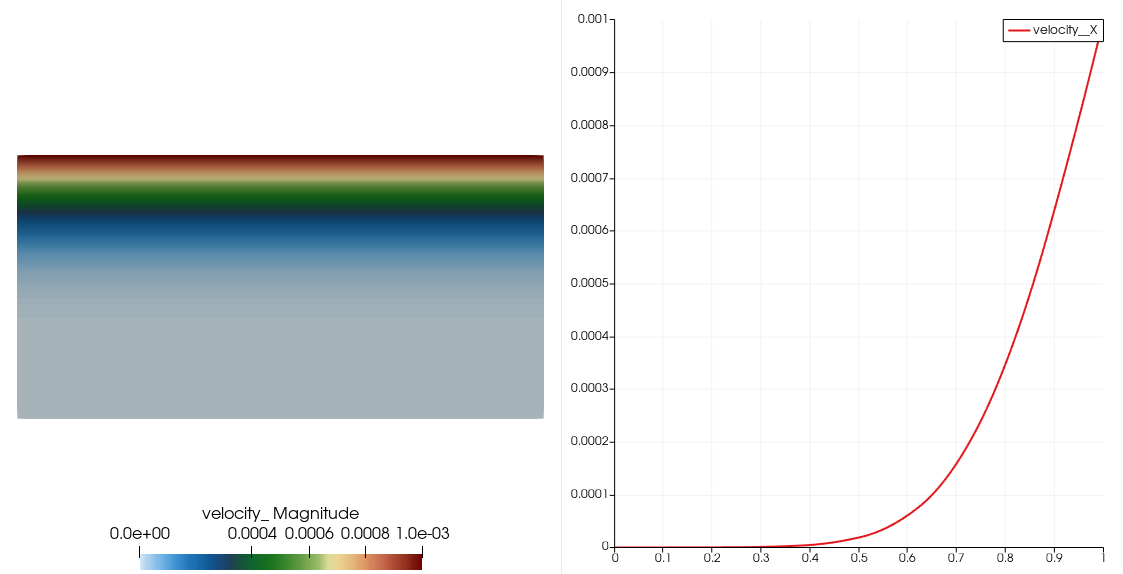
\includegraphics[height=1.2in]{images/2d_quad9_couette_results_early.png}
  }
  \centering
  \subfloat[]
  {
   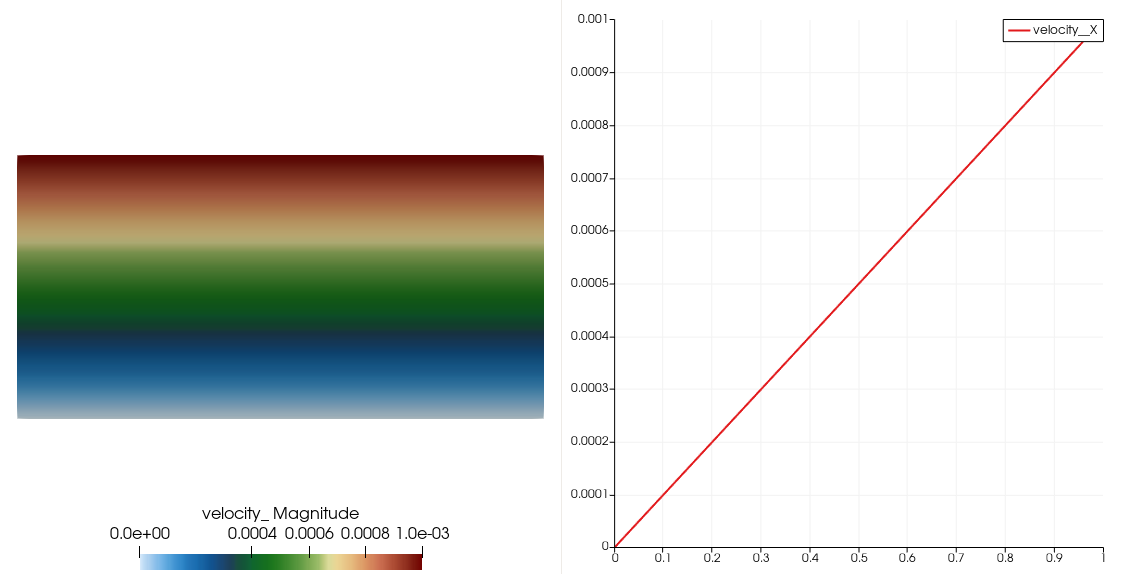
\includegraphics[height=1.2in]{images/2d_quad9_couette_results_late.png}
  }
  \caption{Velocity shadings (left) and velocity profile (right) for the $Re = 1236$ case.}
  \label{fig:results}
\end{figure}

\section{Discussion Points}

There are several interesting activities associated with this sample case including
the following:

\begin{itemize}
	\item Ensure that derivation of Equation~\ref{eq:simpleEqWithoutK} is clear.
	\item Explore the mesh and input file specifications associated with this case.
	\item In Figure~\ref{fig:results}, the flow results demonstrate a linear profile, as 
          expected. Based on past experience with a linear basis, comment on the usage of a quadratic
          basis.
        \item Probe all degree-of-freedom results, i.e., velocity and pressure. What is of interest?
        \item Modify the underlying equation to include a specified constant bouyant force. This will mimic
          a couette flow in a (potentially) adverse pressure gradient configuration. Can you generate
          Figure~\ref{fig:analytical}?
\end{itemize}

\begin{figure}[!htbp]
  \centering
  {
   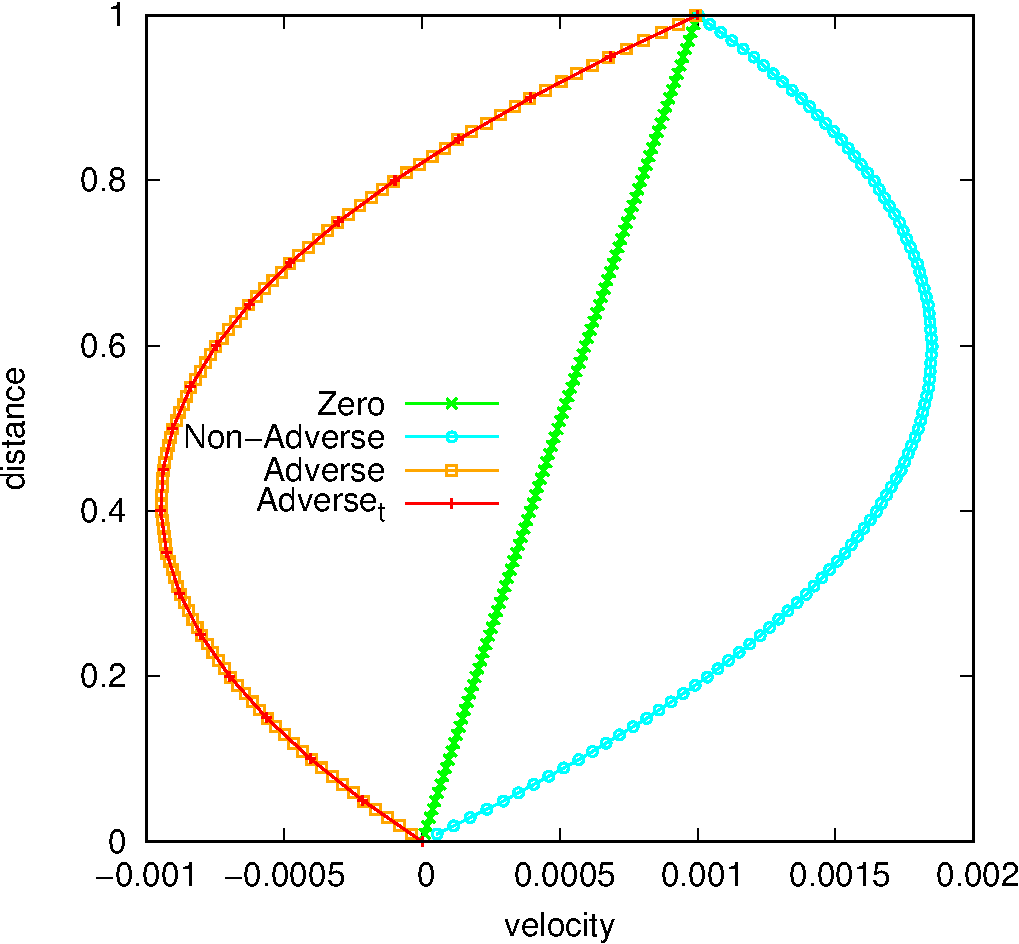
\includegraphics[height=3.0in]{images/couette-crop.pdf}
  }
  \caption{Velocity as a function of height, $u_x(y)$ for a zero, adverse, and non-adverse pressure gradient. For the theoretical
    adverse pressure gradient, a constant body force of magnitude $1.0 \times 10^{-5}$ was applied in addition to the current
    property specification set of values. The above result exercised a linear basis mesh with constant mesh spacing of 0.05.}
  \label{fig:analytical}
\end{figure}

\end{document}
